% CoRA-centered working draft, 2026-09-21.
% Evidence and editorial decisions: PAPER_CORA_NOTES_20260921.md.
% Existing test.tex and all experiment artifacts are preserved.
% Format follows test.tex: article + spconf, with no generic-layout fallback.
% Compile from the repository root. References are embedded below.
\documentclass{article}
% Keep spconf's Times fonts with the local Tectonic/XeTeX compiler.
\usepackage[T1]{fontenc}
\usepackage{spconf,amsmath,amssymb,graphicx,booktabs,algorithm,algorithmic,hyperref}
\usepackage{multirow}
\newcommand{\U}{\mathbf{U}}
\newcommand{\X}{\mathbf{X}}
\newcommand{\HH}{\mathbf{H}}
\newcommand{\C}{\mathcal{C}}
\newcommand{\cora}{CoRA}

\title{CoRA: Randomized Decoding for Quantized Update Inversion\\
and Its Reconstruction Limits Across Bit Widths}
\name{Anonymous Author(s)}
\address{Anonymous Affiliation}

\begin{document}
\maketitle

\begin{abstract}
Quantizing a model update leaves multiple numerical updates compatible with
the transmitted observation. We study \cora{} (Consistency-Ranked restart
Attack), which explores this ambiguity through randomized decoding,
source separation, and feature inversion. The sender quantizes
deterministically; randomness enters only when the attacker samples
admissible values within the observed quantization cells. A public score
combining feature agreement and total variation ranks the resulting
reconstructions, and selected candidates receive further optimization.
We evaluate this procedure on VGG16/ImageNet local updates using signed
per-tensor quantization from 8 to 4 bits. As precision decreases, the
selected reconstruction's LPIPS increases from 0.5558 to 0.8085 and PSNR
decreases from 12.0568 to 11.5028 dB. Reconstructions at 8 bits retain
visible structure in some examples, whereas the 4-bit outputs exhibit
substantial loss of object and scene detail. Relative to naive
dequantization, the benefit of randomized decoding varies with bit width
and metric. These results characterize both the behavior and the limits
of \cora{} under the evaluated reconstruction budget.
\end{abstract}

\begin{keywords}
Update inversion, randomized decoding,
quantization, source separation, reconstruction quality.
\end{keywords}

\section{Introduction}
\label{sec:intro}
Model updates can reveal information about the data used to compute them.
Deep Leakage from Gradients and Inverting Gradients reconstruct training
inputs through gradient matching~\cite{zhu2019deep,geiping2020inverting}.
The Cocktail Party Attack (CPA) instead uses
independent component analysis to separate the inputs mixed in fully
connected gradients and updates~\cite{kariyappa2023cocktail}.
In a compressed communication setting, however, an attacker receives a
quantized representation rather than the original numerical update.
The reconstruction procedure must therefore choose how to decode it.

Naive dequantization assigns every received code its cell center. This is
a natural deterministic estimate, but it represents only one numerical
completion of the observation. A randomized decoder can generate other
admissible completions and pass them through the same reconstruction
pipeline. The important empirical questions are whether candidate search
helps recover image structure and how the resulting quality changes when
the quantization cells become wider.

We address these questions with \cora{}, a randomized decoding and
candidate-selection procedure. It samples values inside the observed
cells, separates source features from each sampled update, and inverts
those features into images. A score computable from the public model and
the recovered features determines which candidates receive additional
optimization. The output is one selected reconstruction; source or image
averaging is not part of the evaluated method.

The paper makes three contributions. First, it specifies a
compression-compatible randomized decoder and its integration with a
CPA-based source-separation and feature-inversion pipeline. Second, it
defines a public candidate-ranking procedure and reports its actual
computational budget. Third, it characterizes reconstruction quality
across an 8/7/6/5/4-bit per-tensor sweep, using paired naive-decoding
controls, image metrics, and qualitative reconstructions. Our emphasis
is the observed dependence on bit width, including settings where
randomized search provides little or no improvement.

\section{Observation Model}
\label{sec:observation}
\subsection{Client update and attacker knowledge}
We consider an exposed single-client local update in a federated learning
round. The client starts from public weights and performs full-batch SGD.
The convolutional feature extractor is frozen, while the fully connected
layers are trained. The attacker knows the starting model, batch size,
and local training configuration, and observes the quantized fully
connected updates with their decoding metadata. The attack uses the
first fully connected weight matrix. Training images, labels, true
features, and uncompressed updates are unavailable to the attack and its
candidate selector.

Let $\HH=[\phi(x_1),\ldots,\phi(x_B)]^\top$ contain the frozen features
entering the first fully connected layer. If the gradient at local step
$t$ is $\mathbf{A}_t\HH$, with loss averaging included in
$\mathbf{A}_t$, then the local update is
\begin{equation}
 \U=\mathbf{W}^{(T)}-\mathbf{W}^{(0)}
     =-\eta\left(\sum_{t=0}^{T-1}\mathbf{A}_t\right)\HH.
 \label{eq:mixture}
\end{equation}
This expresses the multi-step update as a mixture of fixed input
features and motivates CPA-based source separation. The sign convention
matches the stored after-training-minus-initial update. Our observation
model does not assume access to an individual update concealed by secure
aggregation.

\subsection{Signed per-tensor quantization}
For each tensor, the deterministic quantizer uses
\begin{equation}
 \begin{aligned}
 Q_b&=2^{b-1}-1,\qquad s=\frac{\|\U\|_\infty}{Q_b},\\
 q_j&=\operatorname{round}_{\mathrm{even}}(U_j/s).
 \end{aligned}
 \label{eq:quantizer}
\end{equation}
Codes lie in $[-Q_b,Q_b]$, giving $2^b-1$ numerical levels, and one
FP32 scale $s$ is stored per tensor. A zero tensor is represented by zero
codes and unit scale. Arithmetic and scale storage follow the FP32
implementation. Throughout this paper, bit width refers to numerical
code precision. The experiment artifacts store codes in int8 with
additional scale and packet metadata; this sweep is not a measurement of
packed communication size.

For positive $s$, the ideal interior cell for code $q_j$ extends from
$s(q_j-\tfrac12)$ to $s(q_j+\tfrac12)$. Ties-to-even rounding,
finite precision, and the requirement to reproduce the tensor scale
determine the actual admissible endpoints. We write $\C(q,s)$ for the
set of FP32 tensors that reproduce the received codes and scale.
Naive decoding uses $U^{\mathrm{ctr}}_j=sq_j$.

\section{CoRA: Randomized Decoding and Candidate Ranking}
\label{sec:cora}
\subsection{Sampling compatible numerical updates}
\cora{} generates candidate first-FC matrices
$\widetilde\U^{(m)}\in\C(q,s)$. For non-anchor coordinates, it
draws uniformly between the admissible cell endpoints and casts to FP32.
An extremal coordinate is anchored to a scale-compatible maximum.
The implementation checks that the resulting matrix reproduces both the
codes and the stored scale under re-encoding. This is a bounded sampling
rule, without a learned or calibrated prior over the original update.

Naive decoding and one randomized draw are different procedures. The
former always returns the cell center; the latter chooses another
compatible value. In the ideal interior-cell model, center decoding has
coordinate error at most $s/2$, whereas a sampled completion can differ
from the true value by almost $s$. Randomization therefore does not
guarantee a more accurate numerical update. Its purpose here is to
explore alternative inputs to the nonlinear reconstruction pipeline.

\subsection{Source separation and feature inversion}
Each decoded first-FC matrix is processed using FastICA initialization
followed by gradient refinement of the source separation. Source rows
are aligned to the center-decoded reference using Hungarian assignment
on absolute cosine similarity. Alignment changes permutation and sign
only; it neither rescales source norms nor averages sources across
members. The absolute recovered sources are used as feature-inversion
targets, denoted $z_{m,i}=|\hat h_{m,i}|$.

For each candidate, feature inversion optimizes images $\hat\X_m$ to
match these targets through the public feature extractor. The
implemented backend is a modified CPA-based pipeline: FastICA and
gradient refinement produce the features, and feature inversion produces
the images. The reported results should be interpreted for this backend.

\subsection{Public screening and continuation}
\label{sec:screen}
After an initial feature-inversion budget, \cora{} computes
\begin{equation}
 J_m=\frac{1}{B}\sum_{i=1}^{B}
 \left[1-\cos\!\left(\phi(\hat x_{m,i}),z_{m,i}\right)\right]
 +0.1\,\mathrm{TV}_{\mathrm{norm}}(\hat\X_m).
 \label{eq:score}
\end{equation}
The score is evaluated on a pixel-boxed clone in normalized model-input
space. It uses only the public model, decoded sources, and current
candidate images. Here, consistency refers to feature agreement,
regularized by total variation; this score does not replay local training
or compare a recompressed image-induced update with the packet.

In the evaluated configuration, $K=8$ sampled candidates each receive
5,000 feature-inversion iterations. The three lowest-scoring candidates
continue to a total of 25,000 iterations, preserving optimizer and
scheduler states. The scheduler horizon is 25,000 from the first step,
and ties use ascending member index. The candidate ranked first at
screening remains the primary reported output after continuation. We do
not choose among the finalists using private image metrics or average
their reconstructions.

This yields the following sequence for a fixed observed packet:
\begin{enumerate}
 \item Decode the center reference and generate $K$ compatible samples.
 \item Separate source features for each decoding and align the sources.
 \item Run initial feature inversion and rank candidates by $J_m$.
 \item Continue the retained candidates and return the originally
       rank-1 candidate at the final optimization budget.
\end{enumerate}
The naive control uses center decoding and the same reconstruction
backend, with 25,000 feature-inversion iterations.

\section{Experimental Evaluation}
\label{sec:experiments}
\subsection{Settings and evaluation protocol}
We evaluate pretrained VGG16 on a fixed ImageNet batch, holding the
victim data and local-training configuration constant across bit widths.
The client uses $B=16$, $T=10$, and SGD learning rate $10^{-3}$, with
zero momentum, zero weight decay, and disabled dropout. Only fully
connected parameters are trained. The quantizer uses one scalar scale
per parameter tensor in every condition.

FastICA uses an iteration cap of 200 and tolerance $10^{-6}$, followed
by 4,000 refinement iterations at learning rate $10^{-3}$. The source
count is $B$. Randomized decoding uses seeds $1234+1000003m$ for
$m=0,\ldots,7$. Feature inversion uses Adam with initial learning rate
0.1 and a cosine scheduler; its feature and total-variation weights are
1 and 0.1. These settings are held fixed across the bit sweep.

We report mean PSNR, SSIM, and VGG-based LPIPS~\cite{zhang2018lpips}.
Higher PSNR and SSIM, and lower LPIPS, indicate better image agreement.
Private evaluation begins only after the public candidate selection has
been fixed. Because source separation is permutation-ambiguous, the
evaluator performs one pixel-MSE Hungarian assignment per candidate and
reuses it for all three metrics and the displayed reconstructions.
LPIPS uses FP32 RGB images mapped from $[0,1]$ to $[-1,1]$.
All reconstructed images contribute to the reported means.

\subsection{Combined compression results}
\label{sec:bits}
\label{sec:cifar100}
% Generated from existing metrics by build_results_table.py; no evaluation.
\begin{table}[!t]
\centering
\caption{Naive versus randomized decoding (PSNR$\uparrow$, SSIM$\uparrow$,
LPIPS$\downarrow$). Dashes denote unavailable results.
Protocols differ between panels (Section~\ref{sec:sparse}).}
\label{tab:compression}
\label{tab:bits}
\small
\setlength{\tabcolsep}{0.8pt}
\renewcommand{\arraystretch}{1.0}
\begin{tabular*}{\columnwidth}{@{\extracolsep{\fill}}lllrrrrr@{}}
\toprule
\multicolumn{8}{l}{\textit{(a) Quantization}}\\
Dataset & Method & Metric & 8-bit & 7-bit & 6-bit & 5-bit & 4-bit\\
\midrule
\multirow{6}{*}{CIFAR-100} & \multirow{3}{*}{Baseline} & PSNR & 11.792 & 11.676 & 12.057 & 11.874 & 11.990\\
 &  & SSIM & 0.1200 & 0.1163 & 0.1203 & 0.1212 & 0.1285\\
 &  & LPIPS & 0.7550 & 0.7469 & 0.7442 & 0.7570 & 0.7372\\
 & \multirow{3}{*}{Random selected} & PSNR & 11.967 & 11.836 & 11.948 & 11.920 & 11.736\\
 &  & SSIM & 0.1090 & 0.1297 & 0.1250 & 0.1244 & 0.1207\\
 &  & LPIPS & 0.7279 & 0.7471 & 0.7429 & 0.7411 & 0.7486\\
\midrule
\multirow{6}{*}{ImageNet} & \multirow{3}{*}{Naive} & PSNR & 12.06 & 11.80 & 11.64 & 11.55 & 11.52\\
 &  & SSIM & 0.2924 & 0.2764 & 0.2596 & 0.2620 & 0.2921\\
 &  & LPIPS & 0.5594 & 0.6118 & 0.6961 & 0.7826 & 0.8071\\
 & \multirow{3}{*}{\cora{}} & PSNR & 12.06 & 11.83 & 11.67 & 11.55 & 11.50\\
 &  & SSIM & 0.3070 & 0.2827 & 0.2690 & 0.2558 & 0.2576\\
 &  & LPIPS & 0.5558 & 0.6332 & 0.6659 & 0.7490 & 0.8085\\
\bottomrule
\end{tabular*}
\par\smallskip
\begin{tabular*}{\columnwidth}{@{\extracolsep{\fill}}lllrrrrr@{}}
\toprule
\multicolumn{8}{l}{\textit{(b) Sparsification: retained fraction}}\\
Dataset & Method & Metric & 80\% & 50\% & 30\% & 20\% & 10\%\\
\midrule
\multirow{6}{*}{CIFAR-100} & \multirow{3}{*}{Baseline} & PSNR & 11.994 & 12.020 & 11.948 & 11.793 & 11.757\\
 &  & SSIM & 0.1289 & 0.1304 & 0.1293 & 0.1266 & 0.1285\\
 &  & LPIPS & 0.7480 & 0.7528 & 0.7351 & 0.7467 & 0.7438\\
 & \multirow{3}{*}{Random selected} & PSNR & 11.994 & 11.911 & 11.845 & 11.812 & 11.855\\
 &  & SSIM & 0.1289 & 0.1306 & 0.1281 & 0.1145 & 0.1119\\
 &  & LPIPS & 0.7480 & 0.7424 & 0.7438 & 0.7432 & 0.7299\\
\midrule
\multirow{6}{*}{ImageNet} & \multirow{3}{*}{Naive} & PSNR & --- & 22.29 & 22.14 & 21.87 & 21.53\\
 &  & SSIM & --- & 0.3344 & 0.3141 & 0.2906 & 0.2631\\
 &  & LPIPS & --- & 0.4864 & 0.5098 & 0.5536 & 0ㅇㅇ323\\
 & \multirow{3}{*}{Random fill} & PSNR & --- & --- & --- & --- & 21.51\\
 &  & SSIM & --- & --- & --- & --- & 0.2610\\
 &  & LPIPS & --- & --- & --- & --- & 0.6300\\
\bottomrule
\end{tabular*}
\end{table}


Table~\ref{tab:compression} groups methods by dataset and presents
compression settings as columns, with separate quantization and
sparsification blocks for CIFAR-100 and ImageNet.
The CIFAR-100 entries report the supplied baseline and random-selected
results. The measured ImageNet
blocks use different attack and evaluation protocols, specified below,
so their absolute scores are not a controlled comparison of the two codecs.

In the ImageNet quantization block, selected \cora{} LPIPS increases from 0.5558
at 8 bits through 0.6332, 0.6659, and 0.7490 to 0.8085 at 4 bits.
PSNR decreases from 12.0568 to 11.5028 dB, while SSIM is not monotonic.
Relative to naive decoding, \cora{} improves SSIM and LPIPS at 8 bits
with nearly unchanged PSNR, and all three metrics at 6 bits. The changes
at 7 and 5 bits are mixed; at 4 bits, all three metrics worsen.

\begin{figure}[!t]
\centering
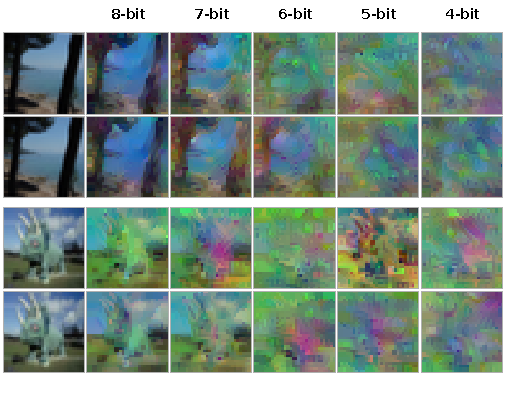
\includegraphics[width=\columnwidth]{paper_assets/quantization_cifar100_imagenet.pdf}
\caption{Paired reconstructions at all five bit widths.
Top four rows: CIFAR-100; bottom four: ImageNet.
The first column shows originals. Within each two-row pair, Naive is
above Random. CIFAR-100 examples are selected post hoc from 24 supplied
examples with $R=8$ outputs; ImageNet examples are fixed independently
of quality, using publicly selected \cora{} after 25,000 FIA iterations.
Saved pairings are preserved, including pixel-MSE matching for ImageNet.
These qualitative cases do not establish a full-set advantage.}
\label{fig:bits}
\label{fig:qualitative}
\end{figure}

\subsection{Sparsification: naive and random filling}
\label{sec:sparse}
The sparsification block uses a separate matched ImageNet study with
frozen convolutional features and the same $B=16$, $T=10$ local-training
configuration. The first-FC update retains its largest-magnitude entries
at keep fractions of 50, 30, 20, and 10\%; naive decoding fills the
remaining entries with zero. These runs use the original CPA optimizer
for 25,000 iterations and FIA for 25,000 iterations. Offline evaluation
uses the saved source-cosine Hungarian assignment for all image metrics,
rather than the pixel-MSE assignment used in the quantization block.

At 10\% retention, a separate randomized procedure fills only discarded
entries uniformly in $[-\tau,\tau]$, where $\tau$ is the smallest retained
magnitude. Retained entries remain unchanged. Twenty candidates each
receive CPA for 25,000 iterations and FIA for 5,000 iterations. An
observable update-consistency score selects three candidates to continue
FIA to 25,000 total iterations, then selects one final whole-batch output.
The score replays the known local SGD procedure using public-model
predicted labels, recompresses the update, and measures its relative
$\ell_2$ discrepancy from the received packet. This selector and backend
differ from the quantization \cora{} configuration.

Naive LPIPS increases from 0.4864 at 50\% retention to 0.6323 at 10\%.
For these updates, 50\% retention removes only already-zero coordinates.
At 10\%, random filling gives LPIPS 0.6300, PSNR 21.5104 dB, and SSIM
0.2610, versus 0.6323, 21.5305 dB, and 0.2631 for naive decoding.
The change is small and mixed. Matched ImageNet random-fill results at the
other retention levels are unreported and remain blank in the table and figure.

\begin{figure}[!t]
\centering
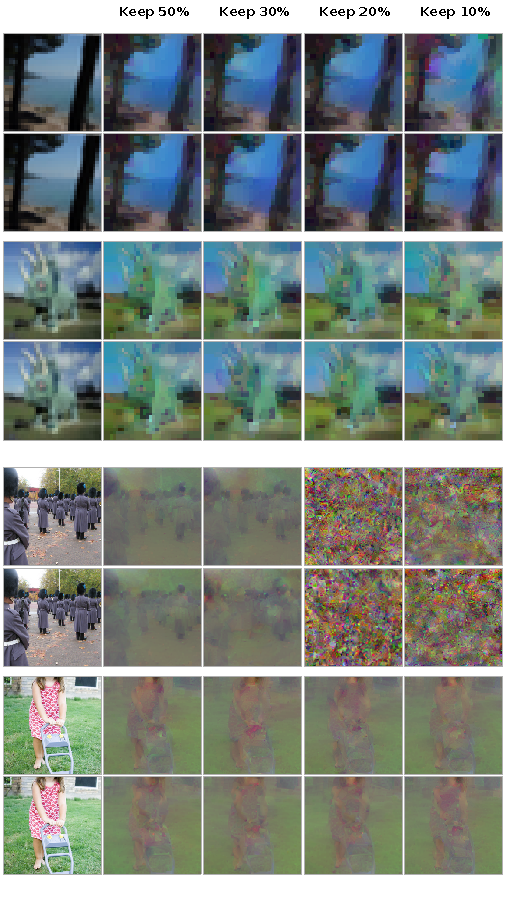
\includegraphics[width=\columnwidth]{paper_assets/sparsification_cifar100_imagenet.pdf}
\caption{Paired sparsification reconstructions at each retained fraction.
Top four rows: CIFAR-100; bottom four: ImageNet. The first column shows
originals; each two-row pair shows Naive above Random.
CIFAR-100 uses the same selected examples as Fig.~\ref{fig:bits}
with supplied $R=8$ outputs. ImageNet uses fixed examples from the
matched same80 study, with zero-fill Naive and publicly selected
$R=20$ Random. Stored pairing is preserved. N/A marks unavailable
matched ImageNet Random results outside 10\% retention. The protocols
differ, so this is not a controlled cross-dataset comparison.}
\label{fig:sparse}
\end{figure}

\subsection{Individual draws and the selected candidate}
\label{sec:individual}
At 4 bits, the first draw (member 00) has PSNR 11.5558 dB, SSIM 0.2614,
and LPIPS 0.8055. It reached the final budget as the third-ranked
candidate, not as a separately evaluated $K=1$ procedure. The public
selector chose member 06, whose image metrics are worse in this example.
Thus public feature agreement is not equivalent to private image
similarity. Table~\ref{tab:compression} retains the publicly selected
candidate rather than replacing it with a more favorable private result.

\subsection{Visual comparison with naive decoding}
\label{sec:qualitative}
Figures~\ref{fig:qualitative} and~\ref{fig:sparse} compare each randomized
output directly with naive decoding of the same observation. The fixed
ImageNet quantization examples include both a poorly recovered image and a person
whose outline is visible at higher precision but deteriorates at lower
precision. The sparse examples show the effect of reducing retention and
the close visual agreement of the two methods at 10\% retention.
These examples supplement the full-set mean metrics; they do not define
a universal reconstruction cutoff.

The CIFAR-100 rows in Fig.~\ref{fig:qualitative} use supplied examples
11 and 24 (one-based display indices), selected after viewing all 24
examples rather than fixed before evaluation. These cases illustrate
differences in retained scene structure at lower precision; fine detail
remains limited and the contrast varies with bit width. All five bit
widths are shown for both methods. Whole image tiles and their saved
pairing are retained without enhancement, averaging, or candidate
reselection. This qualitative selection does not change the aggregate
results or establish a general low-bit recovery advantage.

\subsection{Computational budget and scope}
\label{sec:budget}
The recorded randomized search performs
$8\times5{,}000+3\times20{,}000=100{,}000$ feature-inversion iterations
per bit width. The separate naive control adds 25,000 iterations,
bringing the recorded total to 125,000. Source separation is performed
for each of the eight samples and for the center reference. Thus final
per-candidate iteration counts match, while total search budgets do not.
The comparison measures the outputs of these procedures; it does not
establish a compute-matched advantage from randomized decoding alone.
For the sparse random-fill comparison, per-batch work is 500,000 CPA
iterations, 160,000 FIA iterations, and 23 local-update replays, versus
25,000 CPA and 25,000 FIA iterations for naive decoding. Its total search
budget is likewise unmatched.

The quantization sweep holds one victim batch and one set of candidate seeds fixed.
It characterizes this setting, without estimating variability across
independent batches or complete search runs. Comparisons to other
datasets, quantization granularities, source-separation backends, or
image-matching protocols require separate evidence.

\section{Discussion}
\label{sec:discussion}
Lower precision widens the numerical ambiguity available to the attacker,
but the additional possible completions do not supply information about
which one matches the private update. Equation~\ref{eq:mixture} also
imposes source structure that independent cell sampling does not
explicitly enforce. Coarse completions can therefore provide poor
inputs to source separation even when they reproduce the packet.
This is a possible explanation of the observed degradation, not a
mechanism isolated by the current sweep.

Candidate ranking presents a second limitation. The feature targets in
Eq.~\ref{eq:score} are themselves estimated from the compressed update.
A reconstruction may fit those targets without resembling the private
image, as the individual-candidate comparison illustrates. In addition,
exact re-encoding of a sampled numerical update does not establish that
local training on the final reconstructed images would reproduce the
same packet. That image-induced update constraint was not evaluated in
the quantization sweep; the separate sparse study uses update replay
for candidate ranking.

The results consequently support a conditional account of reconstruction
limits: with this sampler, selector, backend, and budget, 8-bit outputs
retain structure in some examples, and lowering precision to 4 bits
substantially degrades that structure. The intermediate-bit measurements
describe the quality trajectory. They do not establish that any bit
width protects against other attack procedures or larger search budgets.

\section{Related Work}
\label{sec:related}
Optimization-based gradient inversion reconstructs inputs by matching
observed and synthetic gradients~\cite{zhu2019deep,geiping2020inverting}.
CPA instead treats fully connected gradients as a blind source separation
problem solved by ICA, enabling reconstruction at larger batch
sizes~\cite{kariyappa2023cocktail}. Zhang et al.~\cite{zhang2022survey}
survey gradient inversion attacks and defenses, including gradient
protection strategies, and organize the main attack paradigms and
reconstruction techniques.

Compression and other forms of gradient obfuscation have also been
examined as defenses. Yue et al.~\cite{yue2023gradient} demonstrate that
image information can remain recoverable after quantization,
sparsification, or perturbation, and caution against treating privacy
as a byproduct of gradient compression. Li et al.~\cite{li2022ggl}
introduce Generative Gradient Leakage, using a GAN prior learned from
public images to reconstruct inputs under gradient degradation.
Ding et al.~\cite{ding2024compressed} target sparsified gradients with
Deep Leakage from Compressed Gradients (DLCG), which compresses synthetic
gradients during reconstruction to account for the observed sparsity.

\cora{} studies randomized decoding and public candidate selection
without introducing a pretrained generative prior. The sender's
quantization is deterministic; the attacker samples alternative numerical
updates compatible with the observation. For quantization, candidates
share a CPA-based reconstruction backend and are ranked by feature
agreement and total variation. The separate sparsification study uses
update-consistency ranking. Our evaluation compares these randomized
procedures with naive decoding across bit widths and retention levels,
reporting reconstruction quality and the actual search budgets.
It characterizes the measured benefits and limits of candidate search
under the evaluated protocols.

\section{Conclusion}
\cora{} reconstructs quantized local updates by sampling compatible
decodings and ranking the resulting image candidates using a public
feature-based score. Its per-tensor VGG16/ImageNet bit sweep shows
decreasing PSNR and worsening LPIPS from 8 to 4 bits, accompanied by a
substantial loss of visual structure. Randomized decoding offers mixed
improvements over naive dequantization and does not compensate for
coarse quantization in the evaluated 4-bit setting. The measured quality
curves and reconstructions describe where the current procedure retains
image information and where its limitations become pronounced.

\begin{thebibliography}{9}
\bibitem{zhu2019deep}
L. Zhu, Z. Liu, and S. Han,
``Deep leakage from gradients,''
in \emph{Advances in Neural Information Processing Systems}, vol. 32, 2019.
% https://papers.neurips.cc/paper_files/paper/2019/hash/60a6c4002cc7b29142def8871531281a-Abstract.html

\bibitem{geiping2020inverting}
J. Geiping, H. Bauermeister, H. Dr\"oge, and M. Moeller,
``Inverting gradients---How easy is it to break privacy in federated learning?,''
in \emph{Advances in Neural Information Processing Systems}, vol. 33, 2020.
% https://papers.neurips.cc/paper_files/paper/2020/hash/c4ede56bbd98819ae6112b20ac6bf145-Abstract.html

\bibitem{kariyappa2023cocktail}
S. Kariyappa, C. Guo, K. Maeng, W. Xiong, G. E. Suh,
M. K. Qureshi, and H.-H. S. Lee,
``Cocktail Party Attack: Breaking aggregation-based privacy in federated
learning using independent component analysis,''
in \emph{Proc. International Conference on Machine Learning},
vol. 202, pp. 15884--15899, 2023.
% https://proceedings.mlr.press/v202/kariyappa23a.html

\bibitem{zhang2018lpips}
R. Zhang, P. Isola, A. A. Efros, E. Shechtman, and O. Wang,
``The unreasonable effectiveness of deep features as a perceptual metric,''
in \emph{Proc. IEEE Conference on Computer Vision and Pattern Recognition},
2018.
% https://openaccess.thecvf.com/content_cvpr_2018/html/Zhang_The_Unreasonable_Effectiveness_CVPR_2018_paper.html

\bibitem{zhang2022survey}
R. Zhang, S. Guo, J. Wang, X. Xie, and D. Tao,
``A survey on gradient inversion: Attacks, defenses and future directions,''
in \emph{Proc. International Joint Conference on Artificial Intelligence},
pp. 5678--5685, 2022.
% https://www.ijcai.org/proceedings/2022/791

\bibitem{yue2023gradient}
K. Yue, R. Jin, C.-W. Wong, D. Baron, and H. Dai,
``Gradient obfuscation gives a false sense of security in federated learning,''
in \emph{Proc. USENIX Security Symposium}, pp. 6381--6398, 2023.
% https://www.usenix.org/conference/usenixsecurity23/presentation/yue

\bibitem{li2022ggl}
Z. Li, J. Zhang, L. Liu, and J. Liu,
``Auditing privacy defenses in federated learning via generative gradient leakage,''
in \emph{Proc. IEEE/CVF Conference on Computer Vision and Pattern Recognition},
pp. 10132--10142, 2022.
% https://openaccess.thecvf.com/content/CVPR2022/html/Li_Auditing_Privacy_Defenses_in_Federated_Learning_via_Generative_Gradient_Leakage_CVPR_2022_paper.html

\bibitem{ding2024compressed}
X. Ding, Z. Liu, X. You, X. Li, and A. V. Vasilakos,
``Improved gradient leakage attack against compressed gradients in federated learning,''
\emph{Neurocomputing}, vol. 608, article 128349, 2024.
% https://doi.org/10.1016/j.neucom.2024.128349
% Replaces the unverified legacy yu2024compressed citation; DLCG targets sparsification.
\end{thebibliography}

\end{document}
